\documentclass{beamer}
\usetheme{Boadilla}
\usefonttheme{professionalfonts}
\usepackage[mathscr]{eucal}
\usepackage{amsmath,amssymb,mathrsfs}
\usepackage{fourier}




\title{parte2}
\author{elena.zazzetti }
\date{November 2019}




\begin{document}




\begin{frame} %#03
	\frametitle{Neal Algorithm 8}
	\begin{itemize}
		\item \textbf{Approach} :
		\begin{itemize}
		    \item Markov chain with permanent state $c$ and $\phi$ %(?)
		    \item Gibbs sampling to the state extended by the addition of $m$ auxiliary parameters \\
		    % No integration with respect $G_{0}$ is required
        \end{itemize}
        \begin{center}
        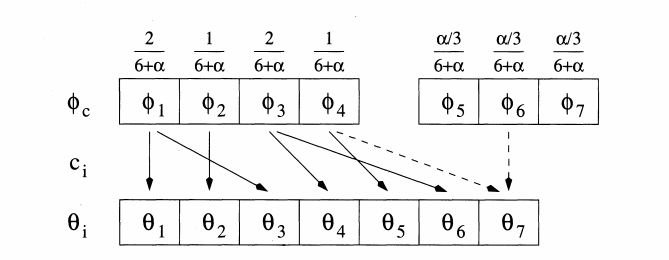
\includegraphics[scale=0.5]{neal.PNG}
        \end{center}
        \item Prior for $c_{i}$ :
            \begin{align*}
                \text{If} \ c=c_{j} \ \text{for some } j: \ P(c_{i}=c | c_{-i}) &= \frac{n_{-i,c}}{n-1-M}  \\
                P(c_{i}\neq c_{j} \text{ for all } j) &=\frac{M }{n-1-M}  \Rightarrow 
                \begin{tabular}{s}
                \textbf{split} among the $m$   \\
                auxiliary parameters 
                \end{tabular}
            \end{align*}
		
	\end{itemize}
\end{frame}




\begin{frame} %#04
	\frametitle{Neal Algorithm 8}
	\textbf{Algorithm}:
		\begin{itemize}
		    \item For $i= 1...n$ : update $c_{i}$  \\
		        \begin{itemize}
		            \item Sample auxiliary parameters: \\ \begin{itemize}
		                \item $c_{i}=c_{j}$ for some $j\ \Rightarrow$ no connection \\
		                \item $c_{i}\neq c_{j} \ \Rightarrow$ association to one of $m$
		            \end{itemize} 

		            The other $\phi$ values drawn from $G_{0}$ \\
		            \item Gibbs sampling update for $c_{i}$: %(by evaluating relative prob of these possibilities)
		                \begin{displaymath}
		                    P(c_{i}=c | c_{-i}, y_{i}, \phi_{1},...,\phi_{h}) \propto \begin{cases}  \frac{n_{-i,c}}{n-1-M}F(y_{i},\phi_{c}), & \mbox{for } 1 \leq c \leq k^{-} \\ \frac{M/m}{n-1-M}F(y_{i},\phi_{c}), & \mbox{for } k^{-}+1 < c \leq h
		                \end{cases}
		                \end{displaymath}
                    \item Discard $\phi$ values not associated
                    
                \end{itemize} 
        
            \item For $c \in \{c_{1},..,c_{n}\}$: update $\phi_{c}$ given $y_{i}$ such that $c_{i}=c$
            
		\end{itemize}
		
\end{frame}


\begin{frame} %#05
	\frametitle{Advantages}
	\begin{itemize}
	    \item  Models with non-conjugate priors
	    \item As $m \rightarrow \infty $ approaches Algorithm 2 but equilibrium distribution is exact 
	    \item More efficient than similar algorithms (e.g. no-gaps) %not reduced prob to create new cluster
	    \item Hierarchical extensions
	\end{itemize}

	
		
\end{frame}


\begin{frame}[c] %#06
	\begin{center}
stick-breaking
		
		(stelline, immagine)
		
	\end{center}
\end{frame}


\begin{frame} %#07
	\frametitle{Blocked Gibbs}
	\begin{itemize}
	    \item \textbf{Assumption}: finite dimensional prior  $P \sim  \mathscr{P}_{N}(\textbf{a},\textbf{b})$
	
%(main use: approximate DPMmodels by truncating the stick-breaking representation of the DP)\\
        \item Finite number of variables $\Rightarrow$ \textit{blocks of parameters} \\
        \item \textbf{Model}:\\
        \begin{align*}
            (Y_{i}|\mathbf{\Phi},\mathbf{c})&\stackrel{ind}{\sim} F(\phi_{c_{i}}) , \ i=1,..,n \\
            (c_{i}|\mathbf{p})&\stackrel{iid}{\sim}\sum\limits_{k=1}^N \mathit{p_{k}}\delta_{k}(\cdot)\\
            \mathbf{p} &\sim \mathscr{GD}(\textbf{a},\textbf{b}) \\
            \mathbf{\Phi_{c}} & \sim G_{0}
        \end{align*}



	\end{itemize}
\end{frame}




\begin{frame} %#08
	\frametitle{Blocked Gibbs}
\textbf{Algorithm}: \\
Repeatedly drawing values from conditional distributions of the blocked variables:\\

\begin{itemize}
    \item $(\Phi | \textbf{c}, \textbf{Y})$
    \item $(\textbf{c}| \Phi,\textbf{p}, \textbf{Y})$
    \item $(\textbf{p}| \textbf{c})$

\end{itemize}

\textbf{Direct sampling of the posterior} $\mathscr{P}(\cdot|\mathbf{Y})$ :\\

\begin{itemize}
    \item The Algorithm produces draws from $(\Phi,\textbf{c},\textbf{p}| \textbf{Y})$ \\
\item Each draw $(\Phi,\textbf{c},\textbf{p})$ defines a measure $P(\cdot)= \sum\limits_{k=1}^N  \mathit{p_{k}}\delta_{Z_{k}}(\cdot) $
\item Each $P$ is a draw from $\mathscr{P}(\cdot|\mathbf{Y})$
\end{itemize}




\end{frame}

\begin{frame} %#09
	\frametitle{Advantages}

	\begin{itemize}
	     \item Handles the issue of conjugacy
	    	    % nonconjugate case Metropolis–Hastings for phi

	    \item Good mixing %(block)

	    \item Hierarchical extensions
	\end{itemize}

\end{frame}

\end{document}
